%! TEX root = ../000-main.tex
% 2022-10-07
\section{Support Vector Machines}

\subsection{Linear SVM}
\label{sec:linear-svm}

\begin{equation*}
	D = \{ (x^1,\, y^1),\, \dots,\, (x^n,\, y^n) \} \quad  x^i \in \mathds{R}^d \; y^i \in \{-1,\, 1\} \mid i = 1,\, \dots,\, n
\end{equation*}

The sum is a \emph{binary classification}.

\begin{equation}
	\mathcal{F}_{\text{lim}} = \{x \to f\left(\omega^Tx + b\right),\quad \omega \in \mathds{R}^d, \; b \in \mathds{R} \}
\end{equation}

The equation $\pi : \omega^Tx + b = 0$ defines a hyperplane.
The idea is to predict class $+1$ whenever $\omega^Tx + b \geq 0$ and class $-1$ otherwise.

\begin{definition}{linsep}{}
	% \paragraph{Def: linsep}
	A dataset is \emph{linsep} if:

	\begin{equation*}
		\exists (\omega,\, \omega_0) \in \mathds{R}^d \setminus \{0\} \times \mathds{R}
		\text{ such that: }
		\forall i=1,\,\dots,\,n\quad y^i(\omega^Tx^i +b) > 0
	\end{equation*}
\end{definition}

We assume from now on that $D$ is \emph{linsep}.

\begin{definition}{geometric margin}{}
	The \emph{geometric margin} of a linear
	classifier $f \to \omega^Tx + b$ at a data point $x$ is the
	euclidean distance from $x$ to the hyperplane $\pi$.

	\begin{equation*}
		\gamma(x) = \frac{\|\omega^Tx + b\|}{\lVert\omega\rVert} \tag{geometric margin}
	\end{equation*}
\end{definition}

The geometric margin of a linear classifier on $D$ is the minimum of
these geometric margins over all data points. That is, it is the distance
from the closest point to the hyperplane.

\begin{equation*}
	\gamma = \min_{x \in D} \gamma(x) \tag{geometric margin of a linear classifier}
\end{equation*}

\begin{figure}[H]
	\begin{tikzpicture}
		\begin{axis}[
				domain=0:11,
				xmin=0, xmax=10,
				ymin=0, ymax=10,
				samples=100,
				% axis y line=center,
				% axis x line=bottom,
				xlabel = {$n$},
				legend pos=south east,
				% area style,
				% ticks=none,
			]
			\addplot+[mark=none] {-x + 5};
			\addplot+[mark=none] {x};
			\addlegendentry{\(\pi: \omega^Tx + b = 0\)};
			\addlegendentry{\omega};
		\end{axis}

	\end{tikzpicture}
	\caption{Hyperplane and its normal vector}
\end{figure}

We set into the problem of finding the hyperplane $f$ that minimizes
its geometric margin over the data, $\gamma_{\text{min}}(f)$.

\begin{equation*}
	\max_{(\omega,\, b)}
	\left\{
	\min_{i=1,\,\dots,\, n}
	\frac{| \omega^Tx^i + b |}{\lVert\omega\rVert}
	\right\}
\end{equation*}

\subsection*{Questions}

\begin{enumerate}
	\item Why should we be doing this? ???
	\item Does a solution always exists? Yes
	\item Is the solution unique? Yes
	\item How do we find the solution?

	      The problem boils down to:
	      \begin{align*}
		      \max_{(\omega, b)}
		      \left\{
		      \min_{\substack{i=1,\dots, n                                                  \\ y^i(\omega^Tx^i + b) > 0}}
		      \underbrace{\frac{1}{\lVert\omega\rVert}}_{\text{margin of the solution}}
		      \right\}                                                                      \\
		      \min_{(\omega, b)} \frac{1}{2}\lVert\omega\rVert^2                            \\
		      \text{subject to} \quad y^i(\omega^Tx^i + b) \geq 1 \quad \forall i=1,\dots,n \\
		      \begin{rcases*}
			      \text{convex} \\
			      \text{QP}     \\
		      \end{rcases*} \Rightarrow \text{Solution is unique}
	      \end{align*}

	      \begin{enumerate}
		      \item Convex
		      \item Quadratic Programming (QP)
	      \end{enumerate}

\end{enumerate}

\subsubsection{The dual problem}

The Lagrangian function:

\begin{align*}
	\mathscr{L}(\omega, b, \alpha)                   & = \frac{1}{2}\lVert\omega\rVert^2 - \sum_{i=1}^n \alpha_i \left[ y^i(\omega^Tx^i + b) - 1 \right] \\
	\alpha                                           & = \begin{pmatrix} \alpha_1 \\ \vdots \\ \alpha_n \end{pmatrix}
	\tag{Lagrangian multiplier}                                                                                                                          \\
	\frac{\partial \mathscr{L}}{\partial \omega} = 0 & \Rightarrow \omega = \sum_{i=1}^n \alpha_i y^i x^i \tag{p1}\label{eq:lagp1}                       \\
	\frac{\partial \mathscr{L}}{\partial b} = 0      & \Rightarrow \sum_{i=1}^n \alpha_i y^i = 0 \tag{p2}\label{eq:lagp2}                                \\
	\text{KKT} \begin{pmatrix}
		           \text{Karush} \\
		           \text{Kuhn}   \\
		           \text{Tucker}
	           \end{pmatrix} \text{ conditions}                                                                                                          \\
	\forall i=1,\dots,n \quad \alpha_i \left[ y^i(\omega^Tx^i + b) - 1 \right] = 0 \tag{kkt}\label{eq:kkt}
\end{align*}

\begin{enumerate}
	\item \ref{eq:lagp1} \textrightarrow{} The solution $\omega$ must be a linear combination of the TR data points $x^i$
	\item \ref{eq:lagp2} \textrightarrow{} The sum of the Lagrangian multipliers is the same for both classes.
	\item \ref{eq:kkt} \textrightarrow{} $\alpha_i = 0$  xor $y^i(\omega^Tx^i + b) = 1$
	      \begin{enumerate}
		      \item $\alpha_i = 0$ \textrightarrow{} The data point $x^i$ is not a support vector
		      \item $y^i(\omega^Tx^i + b) = 1$ \textrightarrow{} The data point $x^i$ is a support vector. And coincide with the points on the margins of the hyperplanes.
	      \end{enumerate}
\end{enumerate}

% 2022-10-14

\begin{align*}
	\mathscr{L}_\text{dual}(\alpha) = \sum_{i=1}^n \alpha_i - \frac{1}{2} \sum_{i=1}^n \sum_{j=1}^n \alpha_i \alpha_j y^i y^j (x^i)^T x^j \\
	\text{goal} \quad \max_{\alpha} \mathscr{L}_\text{dual}(\alpha)                                                                       \\
	\text{subject to} \quad
	\begin{rcases*}
		\sum_{i=1}^n \alpha_i y^i = 0 \\
		\alpha_i \geq 0
	\end{rcases*} \quad \forall i=1,\dots,n
\end{align*}

\begin{note}{}{}
	The data points $x^i, i=1,\dots,n$  appear \emph{only} as
	dot products.
\end{note}

\begin{note}{}{}
	The (primal) solution vector $\omega$
	can be expressed as a linear combination of the (known) data points$x^i$.
\end{note}

% How \emph{general} are these properties?

\begin{question}{}{}
	How \emph{general} are these properties?
\end{question}

\begin{question}{What kind of problem do we have?}{}
	Quadratic problem subject to linear (inequality) constraints is
	a \emph{quadratic programming} (QP) problem.
\end{question}

\begin{question}{What is the SVM model?}{}
	We have two versions of the SVM model, the primal and the dual:
	\begin{equation*}
		f_\text{SVM}(x) = \text{sign} \left( \hat{\omega}^T \boldsymbol{x} + \hat{b} \right)
		\quad \hat\omega \in \mathds{R}^d
		\quad b \in \mathds{R}
		\tag{PRIMAL}
	\end{equation*}

	For the primal version, we have $d+1$ parameters to estimate.

	\begin{align*}
		 & = \text{sign} \left( \left(\sum_{i=1}^n \hat\alpha_i y^i x^i \right)^T x + \hat{b} \right) \\
		 & = \text{sign} \left( \sum_{i=1}^n \hat\alpha_i y^i
		\underbrace{(x^i)^T x}_{\text{data}} + \hat{b} \right)
		\tag{DUAL}
	\end{align*}

	For the dual problem, we have $n$ parameters to estimate.
	And the data appears only as dot products.

	\vspace{0.5em}
	We use primal or dual depending on the dataset:
	\begin{enumerate}
		\item If $n \ll d$ we use the primal problem.
		\item If $n \gg d$ we use the dual problem.
	\end{enumerate}
\end{question}

\begin{question}{What kind of model is the dual version of $f_\text{SVM}$}{}
	\begin{itemize}
		\item linear
		\item non-parametric (see def.~\ref{def:parametric})
		\item discriminative (see def.~\ref{def:discriminative})
	\end{itemize}
\end{question}

\begin{definition}{Parametric model}{parametric}
	A model is called \emph{parametric} when its size does not
	grow with the size of the training data.

	\begin{enumerate}
		\item size of the model = number of free parameters (unknowns)
		\item size of the training data = $n$
	\end{enumerate}
\end{definition}

\begin{definition}{Leave One Out cross-validation error}{loo}
	%TODO
\end{definition}

\begin{theorem}{LOO analysis}{looanal}
	\begin{lemma}{
			The average LOO-CV error $f_n$ data sets sets of size $n \geq 2$
			is an unbiased estimator of the average (true) generalization
			error for data sets of size $n=1$.
		}

		\begin{align*}
			\mathds{E}_{D^n \sim p^n}
			\left[ \hat{R}_{LOOCV}(f_{D_n}) \right] =
			\mathds{E}_{D^{n-1} \sim p^{n-1}} \left[{R_{LOOCV}(f_{D_n})} \right]
		\end{align*}
	\end{lemma}

	Let $f_{D_n}$ as in the lemma, let $SV(f_{D_n})$ be the set of
	support vectors in $D_n$. Then:
	\begin{equation*}
		\mathds{E}_{D^{n-1} \sim p^{n-1}} \left[{R(f_{D_n})} \right]
		\leq \mathds{E} \left[
			\frac{\left| SV(f_{D_n}) \right|}{n + 1}
			\right]
	\end{equation*}

	This is an argument in favor of \emph{sparsity} (def.\ref{def:sparsity}).
\end{theorem}

\begin{definition}{Sparsity}{sparsity}
	The fraction of data points used in the final model.
\end{definition}

\subsection*{Non-separable data}

This means that there is at least one pair of data point $(x^i, y^i)$
such that $\nexists (\omega, b) \mid y^i (\omega^T x^i + b) \ngeq 1$.

The solution is:

\begin{equation*}
	y^i (\omega^T x^i + b) \geq 1 - \xi_i, \quad \xi_i \geq 0,\quad
	i=1,\dots,n
\end{equation*}

These $\xi_i$ variables are called \emph{slack variables}.

$\xi_i$ is the amount needed s.t. $y^i (\omega^T x^i + b) \geq 1$.

The\begin{figure}[H]
	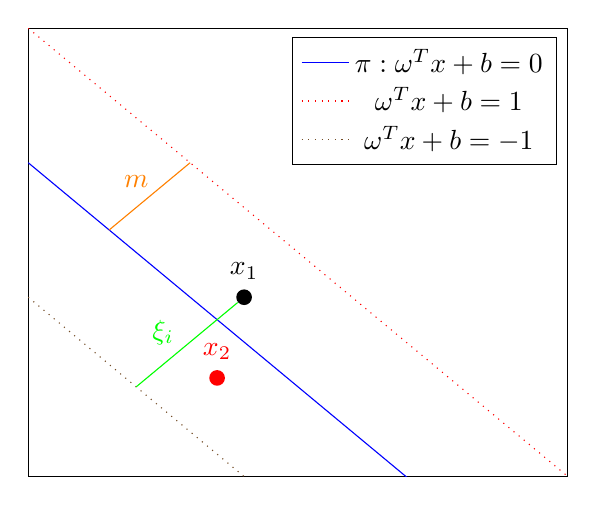
\begin{tikzpicture}
		\begin{axis}[
				domain=0:10,
				xmin=0.0, xmax=10,
				ymin=0, ymax=10,
				samples=100,
				% area style,
				ticks=none,
			]
			\addplot+[mark=none] {7 - x};
			\addplot+[mark=none, dotted] {10 - x};
			\addplot+[mark=none, dotted] {4 - x};
			\addlegendentry{$\pi: \omega^Tx + b = 0$}
			\addlegendentry{$ \omega^Tx + b = 1$}
			\addlegendentry{$ \omega^Tx + b = -1$}
			\node[name=x1,label={90:{$x_1$}},circle,fill,inner sep=2pt] at (axis cs:4,4) {};
			\node[name=x2,label={90,red:{$x_2$}},circle,fill,red,inner sep=2pt] at (axis cs:3.5,2.2) {};
			\draw[orange] (axis cs:3,7) -- (axis cs:1.5,5.5);
			\node[label={90,orange:{$m$}}] at (axis cs:2,6) {};
      \draw[green] (axis cs:2,2) -- (x1);
			\node[label={90,green:{$\xi_i$}}] at (axis cs:2.5,2.5) {};
		\end{axis}

	\end{tikzpicture}
\end{figure}

If we remove the points inside the margin, we get a new dataset
which is linearly separable and has 0 training error. This is called
\emph{soft margin} SVM, in contrast with a hard-margin SVM, and
the margin will be $\frac{2}{\|\omega\|}$.

Finding the hyperplane with the smallest training error
if NP-hard.

We  have two antagonic goals:
\begin{enumerate}
	\item maximize the margin
	\item \textbf{minimize the training error} An upper bound on the
	      number of training errors is upper bounded y the sum of the slacks:
	      \begin{equation*}
		      n TR \leq \sum_{i=1}^n \xi_i
	      \end{equation*}
\end{enumerate}

The new optimization problem is:
\begin{align*}
	\min_{\omega, b, \xi} &
	\underbrace{\frac{1}{2} \|\omega\|^2}_{\text{maximize the margin}}
	+ C \cdot \underbrace{\sum_{i=1}^n \xi_i}_{\text{minimize the TR}} \\
	\text{s.t.}           & \begin{rcases*}
		                        y^i (\omega^T x^i + b) \geq 1 - \xi_i \\
		                        \xi_i \geq 0
	                        \end{rcases*}
	\quad i=1,\dots,n
\end{align*}

We add an hyperparameter $C$ which controls the tradeoff between
these two goals.
